\chapter{Metodologia}
  \section{Gerenciamento}
    \subsection{Estrutura Analítica do Projeto (EAP)}

      Tendo como objetivo a visão geral sobre as atividades que serão
      realizadas no decorrer do projeto, escolheu-se a EAP como forma
      de organização sistematizada das informações.

      A EAP consiste em uma organização das entregas
      a serem feitas em um formato de árvore, partindo de tarefas
      mais gerais para tarefas mais específicas \cite{pmbok2012}.

      Para a construção da EAP, foram levados em conta as diferentes
      entregas a serem realizadas dentro do ciclo de vida do projeto,
      assim como as áreas de atuação dentro da equipe. Além disso, é
      possível observar o alinhamento da EAP com as atividades previstas
      no cronograma e com os requisitos estabelecidos para o projeto.

      A figura \ref{fig:eap} é a representação gráfica da EAP do projeto.

      \begin{figure}[!htbp]
        \centering
        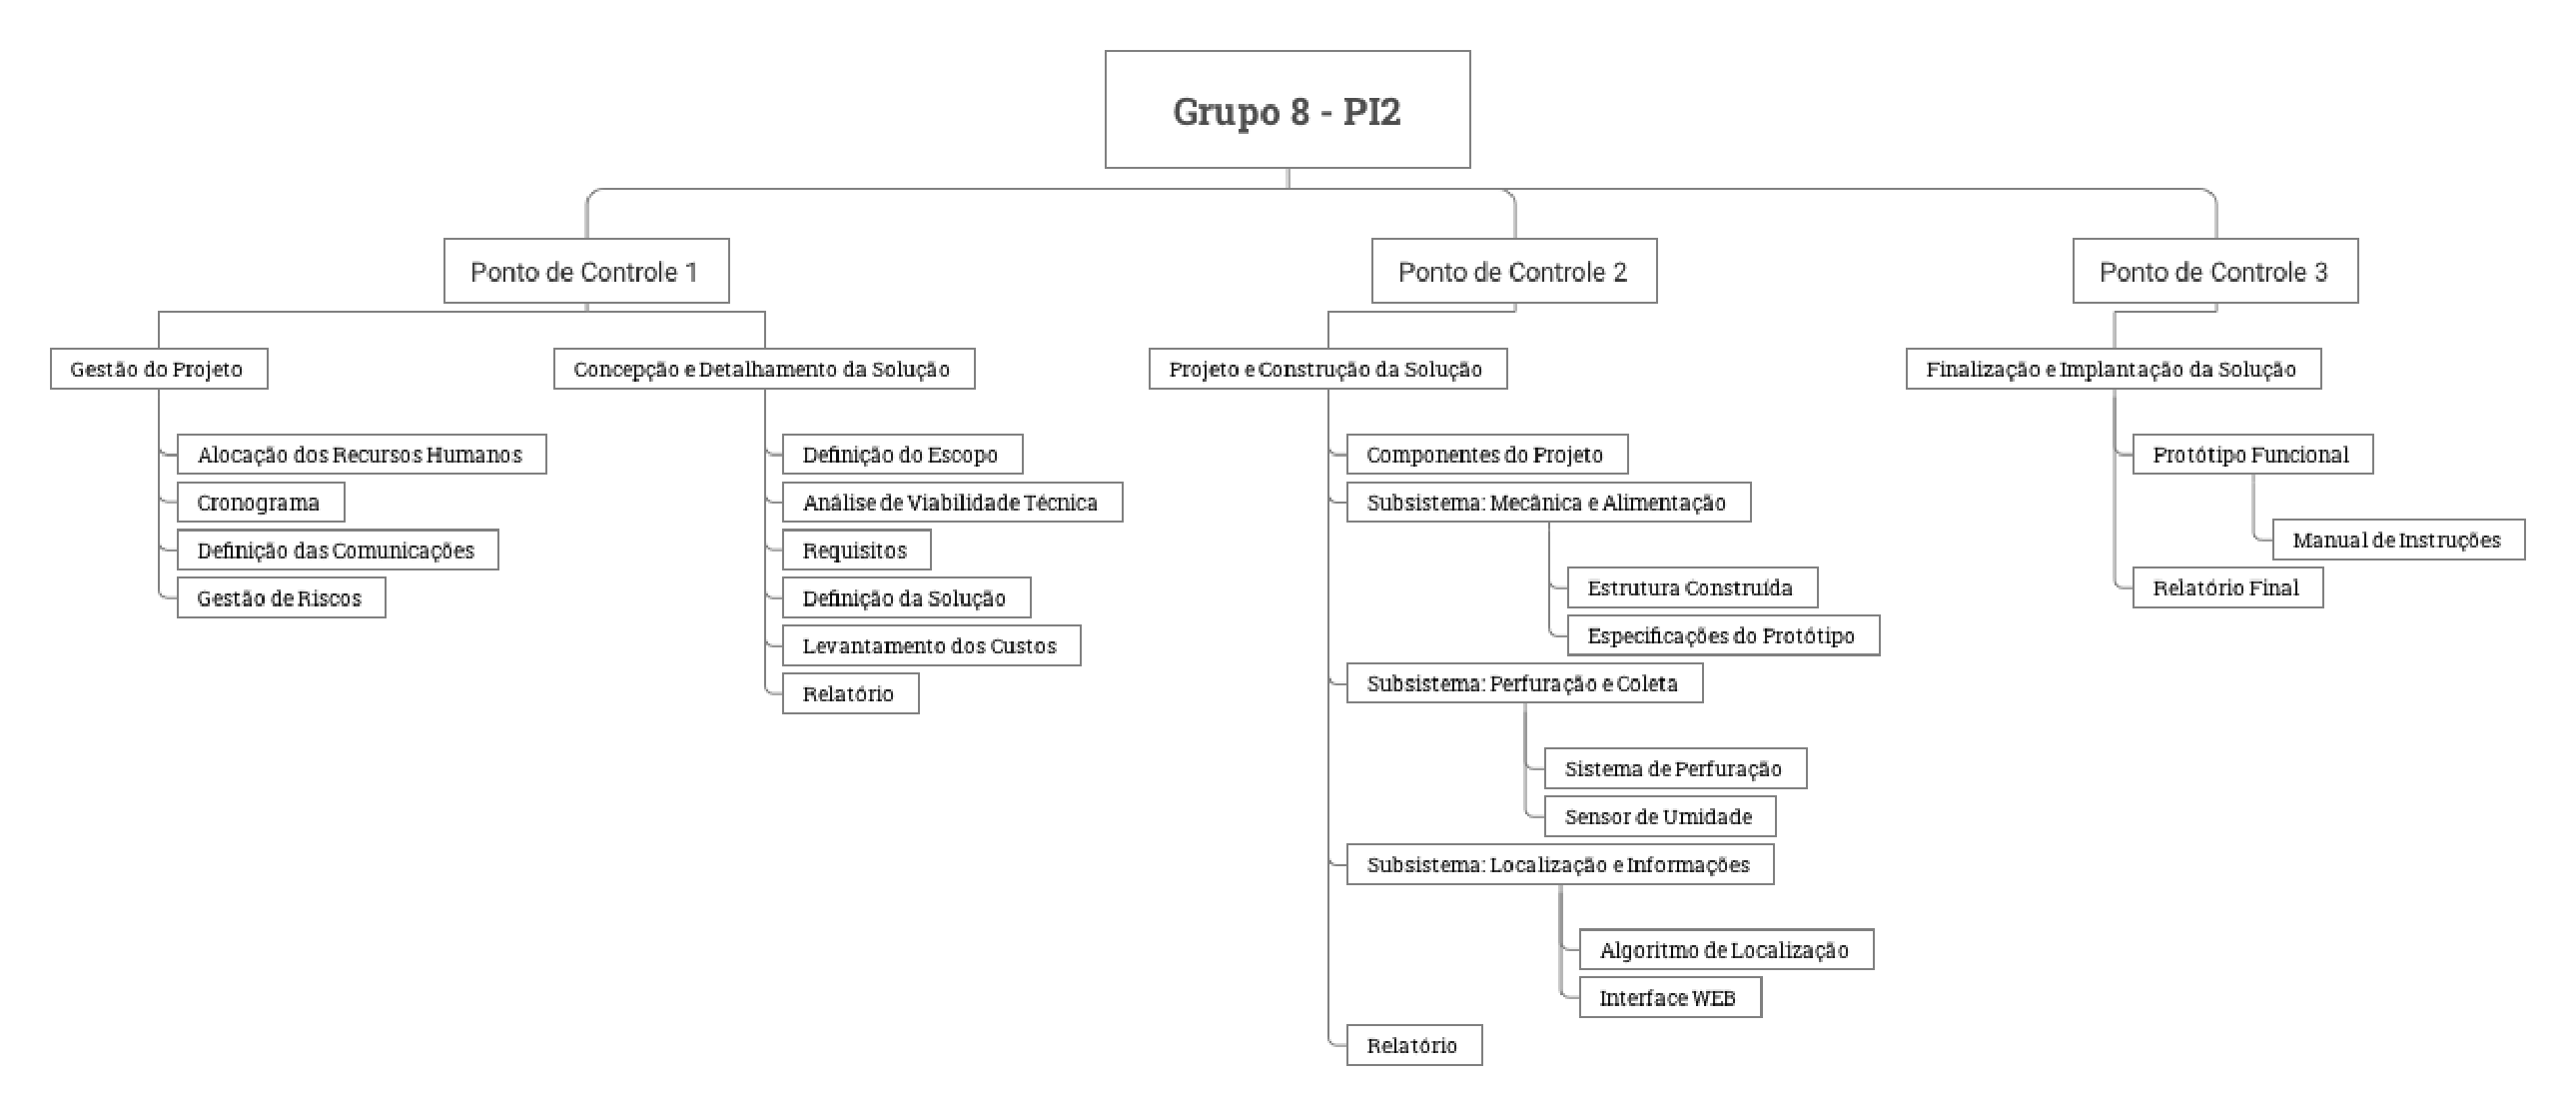
\includegraphics[width=\textwidth]{figuras/EAP.eps}
        \caption{Estrutura Analítica do Projeto. Fonte: autores.}
        \label{fig:eap}
      \end{figure}

      \vfill
      \pagebreak

    \subsection{Alocação dos Recursos Humanos}

      A equipe do projeto, formada por 15 (quinze) integrantes, foi
      subdivida em 3 (três) áreas de atuação, que são: "Mecânica e Alimentação", "Perfuração e Coleta" e "Localização e Informações".

      As áreas são supervisionadas e administradas por uma gestora geral, Jéssica Guimarães,
      e por um gestor da qualidade, Leonardo Cambraia.

      Cada uma das áreas citadas acimas é responsável pela análise de alternativas
      para a solução e a escolha de uma destas para ser aplicada no projeto.

      A figura \ref{fig:aloc} ilustra a estrutura de alocação de recursos humanos do
      projeto. A divisão dos integrantes foi feita levando em conta o
      interesse e conhecimento prévio individual nas áreas propostas.
      É importante salientar que toda a estrutura está sujeita a mudanças, sempre
      visando suprir as necessidades do projeto.

      \begin{figure}[!htbp]
        \centering
        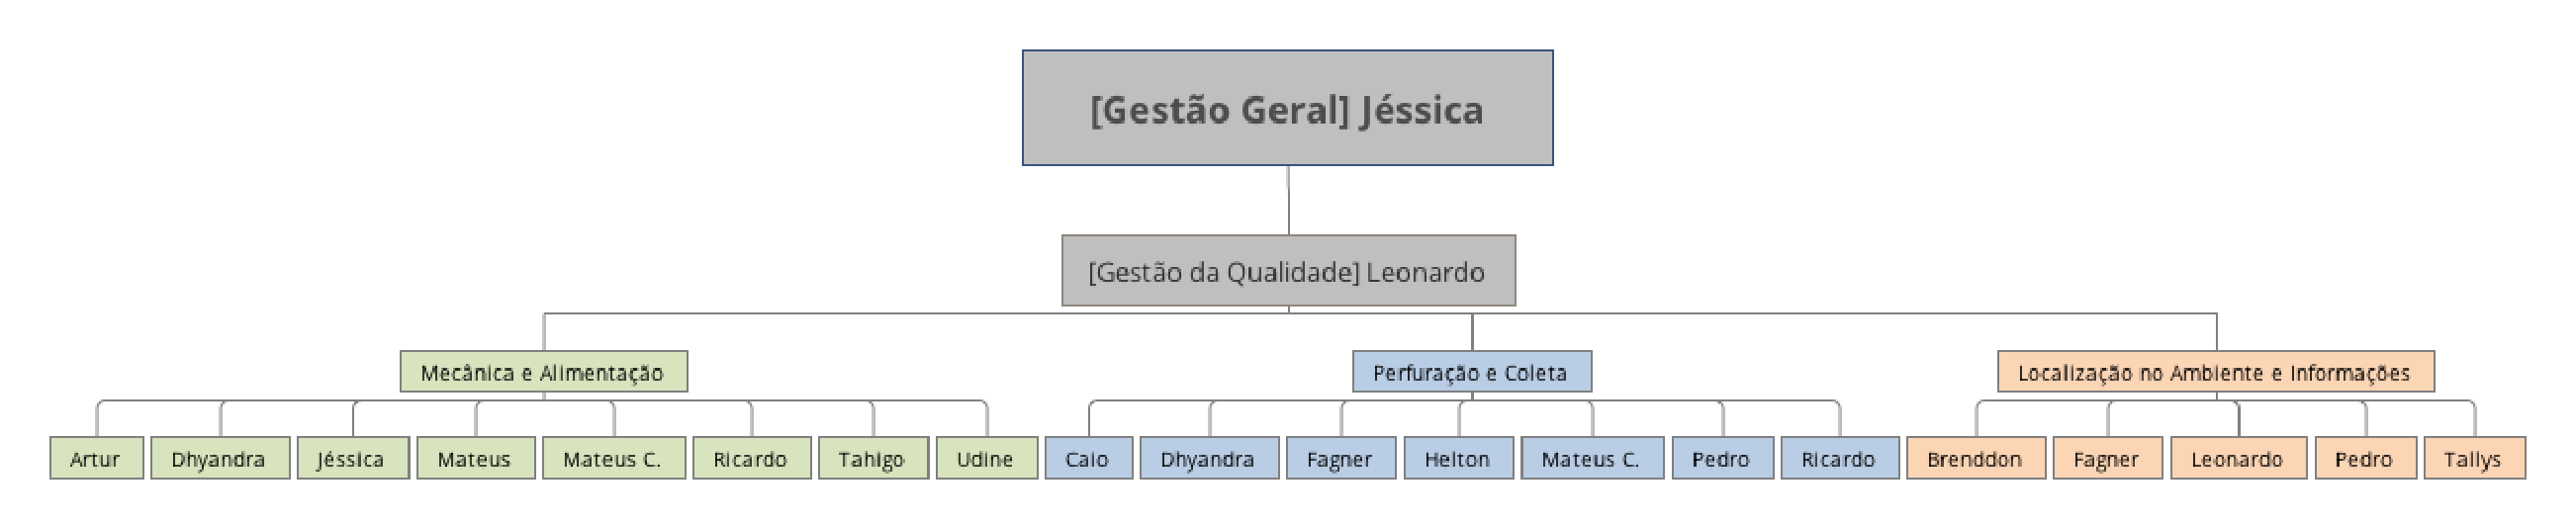
\includegraphics[width=\textwidth]{figuras/alocacao.eps}
        \caption{Alocação de recursos humanos. Fonte: autores.}
        \label{fig:aloc}
      \end{figure}

    \subsection{Comunicação}

      Para que qualquer projeto tenha sucesso é necessário o engajamento da equipe, sendo assim, é necessário uma comunicação eficaz entre os membros da equipe. A tabela \ref{tab:com} detalha os métodos de comunicação utilizados pela equipe.
      
      \begin{table}[!htbp]
      	\begin{center}
      		\caption{\label{tab:com}Métodos de comunicação. Fonte: autores.}
      		\begin{tabular}{|p{4cm}|p{4cm}|p{3cm}|p{3cm}|p{2cm}|}
      			\hline
      			\textbf{Objetivos} & \textbf{Ferramenta} & \textbf{Frequência} & \textbf{Horário} & \textbf{Local}\\\hline\hline
      			Acompanhamento das atividades & Kanban & Sob demanda & Horário da disciplina & FGA\\\hline
      			Avisos rápidos / Lembretes & Telegram & Sob demanda & N/A & N/A\\\hline
      			Decisões Técnicas/Planejamentos & Presencial & Duas vezes por semana & Horário da disciplina & FGA\\\hline
      			Desenvolvimento do projeto & Google Docs/ Google Hangouts/ Git / Github / Presencial & Sob demanda & Durante desenvolvimento do projeto & N/A\\\hline
      		\end{tabular}
      	\end{center}
      \end{table}

    \subsection{Tempo}

      Para a definição das atividades a serem realizadas durante o
      projeto utilizou-se como base os pacotes de trabalho estabelecidos
      na Estrutura Analítica do Projeto (EAP), onde os mesmos foram devidamente
      decompostos com base nos três grandes marcos do projeto referentes
      às entregas de Ponto de Controle 1, 2 e 3. Para tal feito, a equipe,
      tanto de gerência quanto de desenvolvimento precisará cumprir
      as atividades elucidadas no cronograma.

      Após decompostos os pacotes de trabalho da EAP, a equipe
      de gerência reuniu-se para discutir como suas atividades seriam
      executadas, visando tanto uma paralelização de atividades quanto
      o tempo estimado e os recursos necessários para tal.

      Para a determinação do tempo foram utilizadas as
      técnicas de \textbf{Analogia} e \textbf{Decisão em Grupo},
      as quais, segundo o \cite{PMI2012}, representam:

      \begin{itemize}
        \item Analogia: baseia-se em pacotes de trabalho/atividades similares
        de projetos anteriores para estimar a duração dos pacotes de trabalho
        e/ou atividades do seu projeto atual.
        \item Decisão em Grupo: nessa técnica o envolvimento da equipe de projeto
        nas estimativas proporcionam comprometimento da mesma com as
        atividades a serem realizadas.
      \end{itemize}

      O cronograma referente ao nosso projeto encontra-se na figura \ref{fig:cron_s1}
      e \ref{fig:cron_s2} abaixo, contendo seus pacotes de trabalho, atividades e datas. Outro
      cronograma mais detalhado está disposto no Apêndice \ref{schedule_ap}.

      \begin{figure}[!htbp]
        \centering
        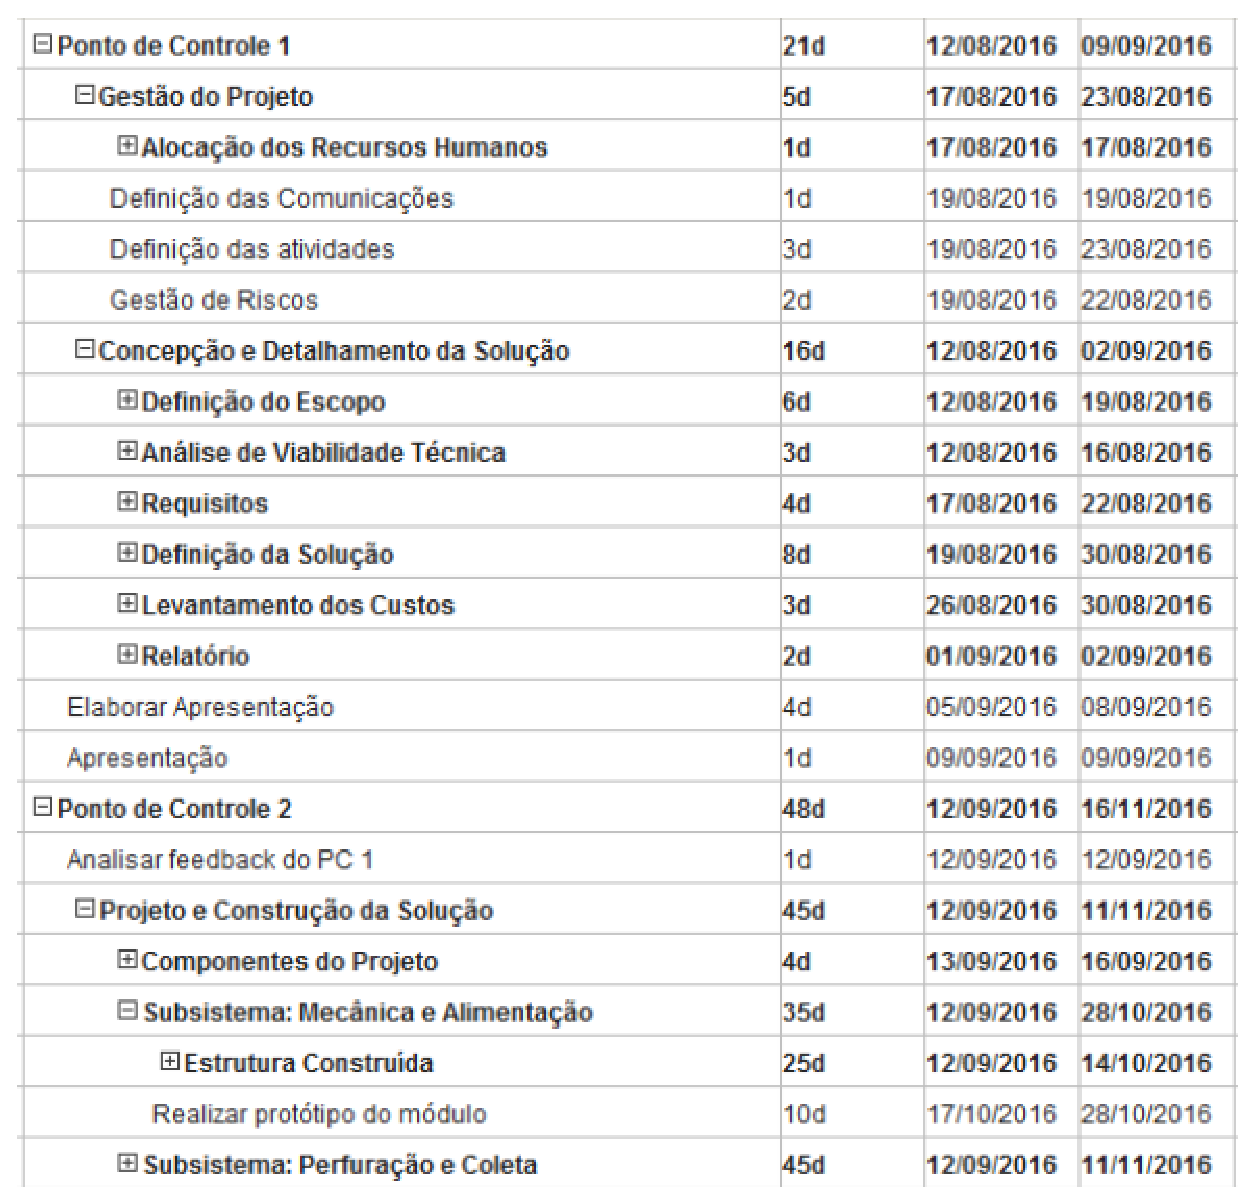
\includegraphics[width=\textwidth]{figuras/cronograma_simples_1.eps}
        \caption{Cronograma de Atividades simplificado (parte 1). Fonte: autores}
        \label{fig:cron_s1}
      \end{figure}

      \clearpage

      \begin{figure}[!htbp]
        \centering
        \includegraphics[width=\textwidth]{figuras/cronograma_simples_2.eps}
        \caption{Cronograma de Atividades simplificado (parte 2). Fonte: autores}
        \label{fig:cron_s2}
      \end{figure}

      \vfill
      \pagebreak
